\documentclass[12pt]{article}
\usepackage{graphicx}
\usepackage{amssymb}
\usepackage{epstopdf}
\usepackage{amsmath}
\usepackage{multicol}
\usepackage{tcolorbox}
\usepackage{geometry}
\usepackage{enumitem}
\usepackage{fancyhdr}

\DeclareGraphicsRule{.tif}{png}{.png}{`convert #1 `dirname #1`/`basename #1 .tif`.png}

\textwidth = 6.5 in
\textheight = 9 in
\oddsidemargin = 0.0 in
\evensidemargin = 0.0 in
\topmargin = -23pt
\headheight = 0.0 in
\headsep = 0.0 in
\parskip = 0.2in
\parindent = 0.0in
\pagestyle{fancy}
\pagenumbering{gobble}

\newtheorem{theorem}{Theorem}
\newtheorem{corollary}[theorem]{Corollary}
\newtheorem{definition}{Definition}
%\includegraphics [height=50mm, width=50mm]{PathInt.jpg}
\title{Title} 

\begin{document}
%INSTRUCTOR NOTES

 Name:
 \begin{center}\large{6.4 Fundamental Theorem of Calculus}\end{center}

Warm-up: Evaluate the following:
\begin{enumerate}
\item $\displaystyle \int (3\sin x + \cos x)\,dx$\\

\item $\displaystyle \int_{-1}^3 |x| \,dx$\\

\item $\displaystyle \int_{-2}^{-1} \frac{x^2+3}{x}\,dx$\\

%\item Find the solution to the initial value problem $y'=1-e^{2x}$, $y(0)=6$.\\
\end{enumerate}

\begin{tcolorbox}
Fundamental Theorem of Calculus:\\

Let $F'(x)=f(x)$, so $F$ is an antiderivative of $f$. Then\\
\begin{enumerate}
\item $\displaystyle \int_a^b f(x)\,dx=$\\

\item $F(x)=$\\
\end{enumerate}
\end{tcolorbox}


\begin{enumerate}
\item Find $F'(x)$ where $\displaystyle F(x)= \int_2^{3x} (2\cos(t))\,dt$\\
\end{enumerate}

\newpage
~

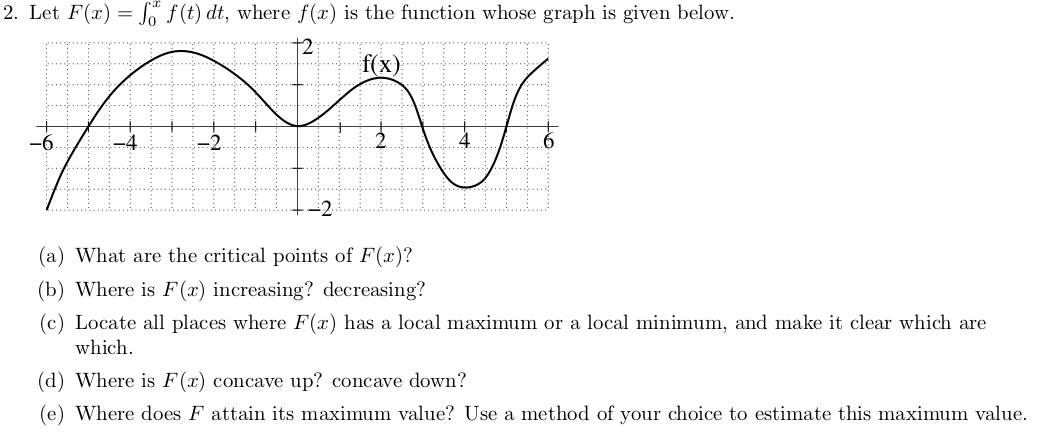
\includegraphics [width=\textwidth]{6_4_FTCa}

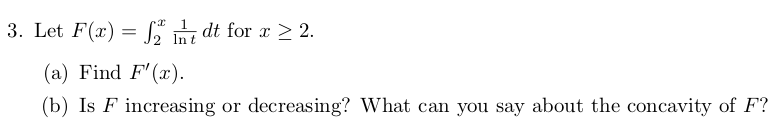
\includegraphics [width=\textwidth]{6_4_FTCb}

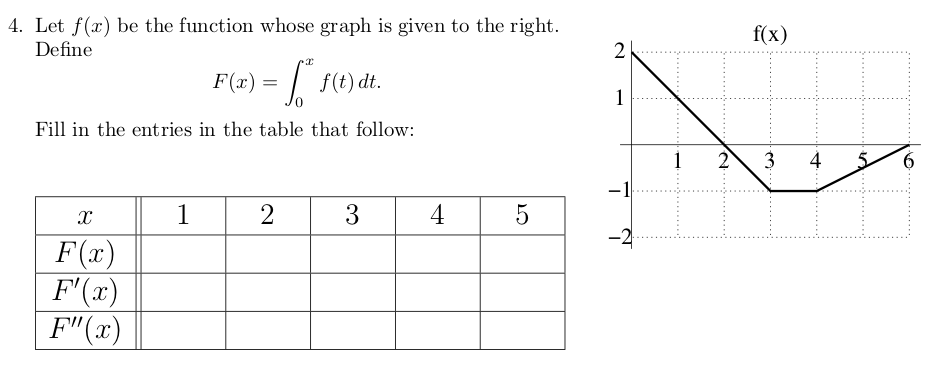
\includegraphics [width=\textwidth]{6_4_FTCc}


\end{document}
%%%%%%%%%%%%%%




